\subsection{Decision Tree Feature Generation}

\subsubsection{MNIST}

In working with the decision trees, we utilized the SVD of each image in the training set. 


\subsection{LDA vs PCA}

LDA and PCA linearly transform the data to reduce the dimensions. The difference between the two techniques is that LDA is supervised whereas PCA is unsupervised. PCA finds orthogonal directions which maximize the variance, thereby expressing the data along \emph{principle components} that are the most pronounced. We can view a PCA technique as in Figure(2.1). 

	\begin{figure}[H]
		\centering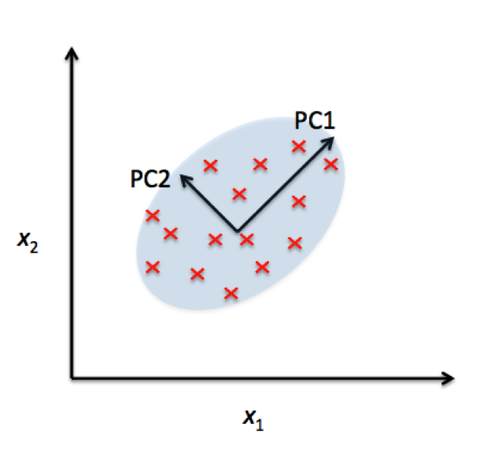
\includegraphics[width=0.4\textwidth]{../images/pca}
		\caption{PCA implemented on 2-dimensional data \cite{images:ldapca}. }
	\end{figure}

LDA maximizes the class separability and can be viewed as in Figure(2.2). 
	\begin{figure}[H]
	\centering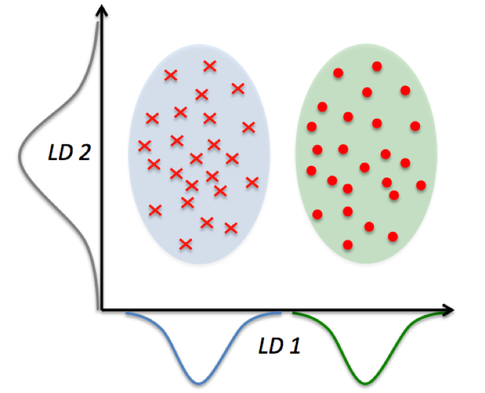
\includegraphics[width=0.4\textwidth]{../images/lda}
	\caption{LDA visualization \cite{images:ldapca}. }
	\end{figure}
The underlying concept of LDA is taking the eigenvectors of $ \dfrac{\Sigma_b}{\Sigma}$ where $\Sigma$ is within-class scatter matrix and $\Sigma_b$ is between-class scatter matrix. By having this division of matrices, we separate the classes away from each other. On the other hand, since PCA is unsupervised it only tries to capture the data in minimum number of variables. 
\subsection{LDA for MNIST and Extended YaleB}
LDA reduces the data with K classes with large dimensions to K-1 dimensions which captures the most energy of the data. Implementing LDA as a dimension reduction, MNIST and Extended YaleB datasets are reduced to 9 and 37 variables for each data point. Then we worked with this transformed data to do further classification. 
